\chapter{РАЗРАБОТКА АНАЛИЗАТОРА ПОСЛЕДОВАТЕЛЬНОСТИ}
\section{Постановка задачи}	



Требуется разработать цифровой узел на основе отладочной платы Digilent Nexys 4,
представляющий собой анализатор фиксированной последовательности логических
сигналов. Узел должен обеспечивать индикацию ожидаемых и вводимых элементов
последовательности посредством входящих в состав отладочной платы семисегментных
индикаторов согласно данному заданию.

Узел должен быть реализован в виде синтезируемой модели на языке Verilog HDL.

Автомат должен иметь интерфейс, представленный на Рисунке~\ref{fig:interface-pract3}.

% TODO: \usepackage{graphicx} required
\begin{figure}[h!]
	\centering
	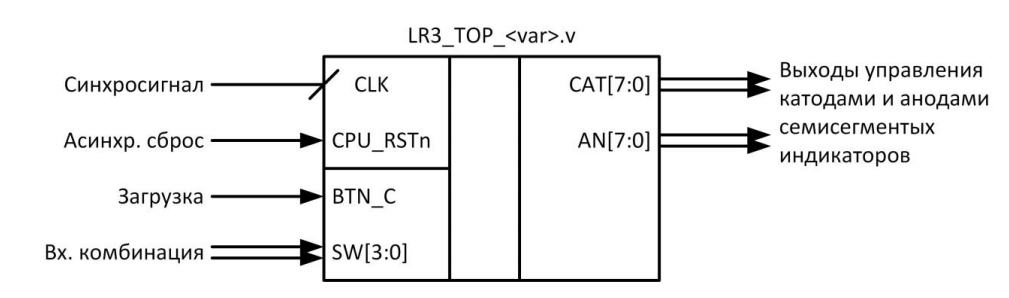
\includegraphics[width=0.7\linewidth]{course-plis/images/lab3/interface-pract3}
	\caption{Интерфейс модели цифрового узла}
	\label{fig:interface-pract3}
\end{figure}


Разрабатываемое устройство является синхронным цифровым узлом,
срабатывающим по восходящим фронтам синхросигнала CLK. Исключение составляет
асинхронный вход сброса CPU\_RSTn, принудительно устанавливающий все регистры
узла в исходное состояние. Подача сигнала сброса на вход узла осуществляется
посредством соответствующей кнопки (CPU\_RSTn) отладочной платы.

Распознавание элементов последовательности осуществляется четверками, т.е.
необходимо обеспечить последовательную загрузку в узел элементов Y c номерами 0-3, 4-
7, 8-B, C-F для успешного распознавания последовательности. При осуществлении ввода
значения, не соответствующего текущему ожидаемому элементу последовательности,
необходимо повторить ввод всей четверки элементов заново




Индикация работы узла посредством двух блоков семисегментных индикаторов подчиняется следующим правилам:
\begin{enumerate}
	\item Левый блок семисегментных индикаторов отображает ожидаемый (младший
	разряд) и введенные (три старших разряда) элементы последовательности в объеме
	распознаваемой четверки.
	\item  Правый блок семисегментных индикаторов отображает предысторию ввода
	комбинаций последовательности. Последняя введенная комбинация отображается в
	младшем разряде блока.
	\item  Не задействованные в текущий момент времени семисегментные индикаторы на
	обоих блоках должны находится в выключенном состоянии.
	\item Обновление отображаемых значений на обоих блоках семисегментных
	индикаторов рекомендуется выполнять с частотой от 60Гц до 200Гц.
\end{enumerate}


\section{Моделирование цифрового устройства}

Реализуем устройство, являющегося синхронным цифровым узлом. Его работу организуем по восходящему фронту синхросигнала, асинхронный сброс --- по нисходящему фронту сигнала CPU\_RSTn. 

Приведем таблицу состояний устройства (см. Таблицу~\ref{tab:states}). Текущее состояние цифрового устройства зависит от последнего введенного пользователем с помощью движковых переключателей элемента последовательности. 

\begin{table}[h!]
	\centering
	\small
	\caption{Состояния цифрового устройства}
	\begin{tabular}{|c|c|c|c|c|c|c|c|c|c|c|c|c|c|c|c|c|c|}
		\hline
		Состояние & 16& 15&	14	&13	&12&11&	10&	9&	8&	7&	6&	5&	4&	3&	2&	1&	0\\ \hline\hline
		Значение & 0 & 4 & 4 & 8 & 3 & 0 & 7 & 2 & 2 & D & 7 & C & 5 & 2 & A & C&-- \\ \hline\hline
		Разряд & F & E & D & C & B & A & 9 & 8 & 7 & 6 & 5 & 4 & 3 & 2 & 1 & 0 &--\\ \hline
	\end{tabular}
	
	\label{tab:states}
\end{table}

Перечислим функциональные узлы, которые уже были реализованы ранее. 

\begin{enumerate}
	\item Делитель частоты. Реализован в разделе~\ref{cha:lab2}.
	\item Фильтр дребезга кнопок. Реализован в разделе~\ref{cha:lab2}.
	\item Конечный автомат генератор последовательности. Реализован в разделе~\ref{cha:lab2}.
\end{enumerate}

Приведем граф состояний цифрового устройства (см. Рисунок~\ref{fig:state-graph-pract3}). Переход в следующее состояние происходит только в случае ввода верного элемента последовательности. При неправильном вводе цифровое устройство переходит в ближайшее пройденное состояние, номер которого кратен 4. Номер состояния, в которое перейдет устройство в случае некорректного ввода можно вычислить по формуле 
\[S_{i+1}=(S_i \div 4) \cdot 4\]

% TODO: \usepackage{graphicx} required
\begin{figure}[h!]
	\centering
	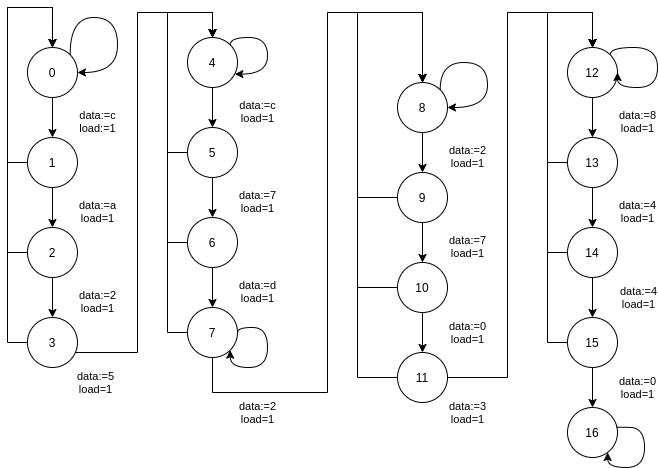
\includegraphics[width=0.7\linewidth]{course-plis/images/lab3/state-graph-pract3}
	\caption{Граф состояний}
	\label{fig:state-graph-pract3}
\end{figure}

%\newpage
Приведем блок схему работы устройства (см. Рисунок~\ref{fig:algorithm-pract3}). Значение Х представляет
собой номер элемента цифровой последовательности, ввод значения которого (Y)
ожидается. Значения Y каждого элемента цифровой последовательности определяются
вариантом задания.

% TODO: \usepackage{graphicx} required
\begin{figure}[h!]
	\centering
	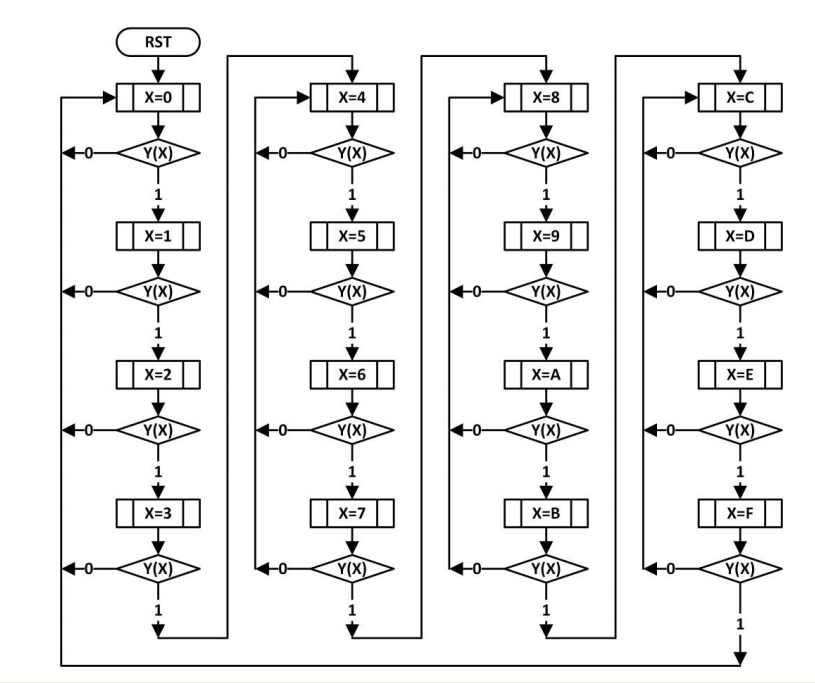
\includegraphics[width=0.68\linewidth]{course-plis/images/lab3/algorithm-pract3}
	\caption{Алгоритм распознавания последовательности}
	\label{fig:algorithm-pract3}
\end{figure}

Приведем структурную схему синхронного цифрового узла (см. Рисунок~\ref{fig:unit-pract3}).

% TODO: \usepackage{graphicx} required
\begin{figure}[h!]
	\centering
	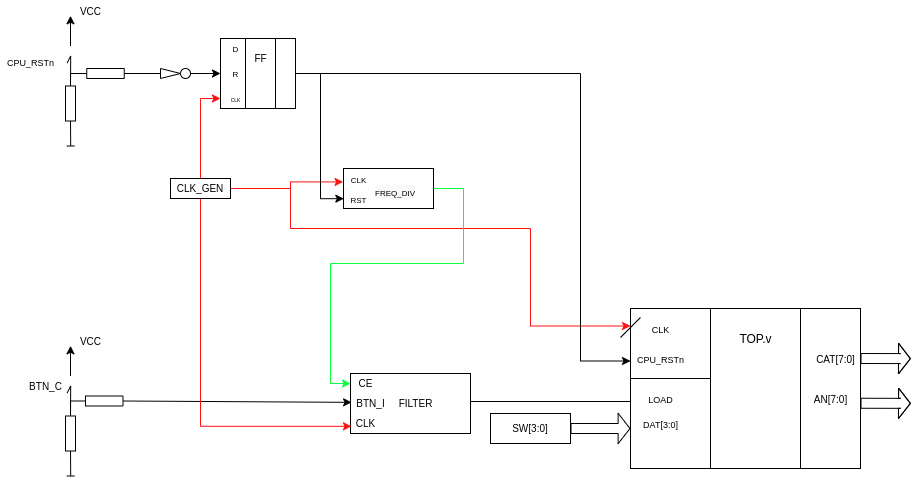
\includegraphics[width=0.8\linewidth]{course-plis/images/lab3/unit-pract3}
	\caption{Структурная схема узла}
	\label{fig:unit-pract3}
\end{figure}


\section{Описание принципа работы}

Опишем главный алгоритм работы цифрового устройства --- контроль ввода шестнадцатеричных чисел с возможностью повторного задания последовательности.

Данный алгоритм описан в файле {seqAuto.v}. Его содержание приведено в приложении~\ref{cha:appendix1} на Листинге~\ref{lst:3seq-auto}.

Сначала производим первоначальную инициализацию переменных, затем, если есть необходимость обновить изображение на дисплее (переменная \texttt{updateDisplay}), начинаем анализировать текущее состояние дисплея и пользовательский ввод. 

Если мы находимся в состоянии, номер которого кратен четырем, то отображаем только левый разряд на левом дисплее. Выводим на это место значение соответствующее значение функции, а в остальные 3 разряда левого дисплея выводим нули.

Если же мы находимся в каком--то другом состоянии, то следует перезаписать все разряды на левом дисплее на один разряд влево, записать в освободившийся разряд записываем очередное значение вектор--функции. 

В конце устанавливаем переменную \texttt{updateDisplay} в нуль. 

Если пользователь подал сигнал на загрузку числа, произведем следующие действия:

Перезапишем все разряды на правом дисплее на один разряд влево, в освободившийся разряд запишем заданное пользователем число. 

Осуществим проверку введенного числа --- сравним его с соответствующим значением вектор--функции. Если пользователь произвел верный ввод, инструментируем переменную состояния автомата (переведем его в следующее состояние). В случае ввода неправильного числа возвращаемся в ближайшее пройденное состояние, номер которого кратен 4. 

В конце устанавливаем переменную \texttt{updateDisplay} в единицу.

\section{Создание проекта САПР Xilinx ISE}

\paragraph{Автомат анализатор входной последовательности.}
Приведем содержание файла seqAuto.v, реализующего главный алгоритм управления цифровым устройством, который был описан в предыдущей секции (см. Приложение~\ref{cha:appendix1} Листинг~\ref{lst:3seq-auto}).


\paragraph{Фильтр дребезга кнопок.}
Используем ранее созданный модуль, реализующий фильтр дребезга кнопок.
Исходный код данного модуля приведен в Приложении~\ref{cha:appendix1} на Листинге~\ref{lst:2filter}.

\paragraph{Делитель частоты.}
Используем ранее созданный модуль, реализующий делитель частоты, применяемый в данном проекте для снижения выходных характеристик частотного генератора для подбора оптимального режима работы с семисегментными индикаторами.
Исходный код данного модуля приведен в Приложении~\ref{cha:appendix1} на Листинге~\ref{lst:2freq-div}.


\paragraph{Драйвер для работы с семисегментыми индикаторами.}
Приведем содержание файла NexysDisplay.v, описывающего работу с семисегментыми индикаторами. Исходный код данного модуля приведен в Приложении~\ref{cha:appendix1} на Листинге~\ref{lst:3display}.

\paragraph{Пользовательская функция.}
Приведем содержание файла outFunc.v, описывающего представление бинарной вектор--функции, значения которой сравниваются с пользовательским вводом. 
Исходный код данного модуля приведен в Приложении~\ref{cha:appendix1} на Листинге~\ref{lst:1beh}.

\paragraph{Сигнальный дешифратор.}
Приведем содержание файла SevenSegDec.v, описывающего работу сигнального дешифратора для работы с семисегментыми индикаторами.
Исходный код данного модуля приведен в Приложении~\ref{cha:appendix1} на Листинге~\ref{lst:3decode}.

\paragraph{Модуль верхнего уровня.}
Приведем содержание файла top.v, описывающего работу модуля верхнего уровня, объединяющего все файлы и организующего работу с устройством.
Исходный код данного модуля приведен в Приложении~\ref{cha:appendix1} на Листинге~\ref{lst:3top}.


\section{Тестирование и отладка средствами симулятора ISim}

Произведем тестирование работы спроектированного цифрового устройства средствами средствами САПР Xilinx ISE 14. 

Результаты тестирования приведены в Приложении~\ref{cha:appendix2} на Рисунках~\ref{fig:3page-1}-\ref{fig:3page-6}.



\section{Вывод}
В данном разделе нами были получены общие навыки работы с программным обеспечением Xilinx ISE Design Suite, изучены основы языка Verilog.

С помощью полученных знаний был спроектирован и разработан цифровой узел на основе отладочной платы Digilent Nexys 4, представляющий собой анализатор фиксированной последовательности логических
сигналов. 


